\chapter{Software Observability}

\begin{tcolorbox}
  \textbf{Observability:} is the ability to
  understand the internal state of
  a system by examining its outputs.
\end{tcolorbox}

Telemetry data - i.e. logs and metrics allows:

\begin{itemize}
  \item detecting possible problems
  \item troubleshooting and handle novel problems (unknown unknowns)
  \item understanding the motivation for system behavior (why is this happening?)
\end{itemize}

\section{OpenTelemetry}

OpenTelemetry is an observability framework and toolkit designed to facilitate
the generation, export and collection of telemetry data such as traces, metrics,
and logs. Open source, as well as vendor- and tool-agnostic.

\subsection{Key concepts}

\begin{itemize}
  \item \textbf{Telemetry}: data emitted by a system during operation, requires instrumentation of the system
  \item \textbf{Service Level Indicator (SLI)}: measures the behavior of the system and en captures the user perspective
  \item \textbf{Service Level Objective (SLO)}: attaches business value to one or more SLIs
\end{itemize}

\subsection{Distributed Tracing}

Distributed tracing observe requests as they propagate
through complex, distributed systems
It is based on three main type of signals: \textbf{Logs}, \textbf{Spans} and \textbf{Traces}.


\subsubsection{Logs}

A log is a timestamped message emitted by services or other
components. Built-in logging facilities in most languages, often lack contextual information.

\paragraph{Log format}


\begin{itemize}
  \item \textbf{Structured}: consistent schema or typed fields, can be JSON or other

  \item \textbf{Unstructured}: don't follow a consistent structure, therefore much more difficult to parse
        and analyze at scale

  \item \textbf{Semistructured}: include machine-readable key/value pairs or delimited fields but do not
        guarantee a stable schema

\end{itemize}

\paragraph{Common Log Format (CLF)} 192.168.1.30 - alice [01/May/2025:07:20:10 +0000] "GET /index.html
HTTP/1.1" 200 9481

\subsection{Span}

A span represents a single unit of work or operation.
Spans describes specific individual operations triggere by a
(user) request. It contains:

\begin{itemize}
  \item name
  \item time-related data
  \item structured log messages
  \item other metadata (i.e. Attributes)
\end{itemize}

\paragraph{Span Kind}

\begin{itemize}
  \item Client: outgoing remote call such as an outgoing HTTP request or database call
  \item Server: incoming remote call such as an incoming HTTP request or remote procedure
        call
  \item Internal: operations which do not cross a process boundary
  \item Producer: creation of a job which may be asynchronously processed later
  \item Consumer: processing of a job created by a producer and may start long after the
        producer span has already ended
\end{itemize}

\subsection{Trace}

A (distributed) trace records the path taken by a single request
as it propagates through multiple services/components.

A trace is made of one or more spans, the first span represents the \textit{root span}.
(span represents a request from start to finish).
The spans underneath the parent provide a more in-depth
context of what occurs.

\section{Context Propagation}


\begin{center}
  \begin{minipage}{0.47\linewidth}
    All spans part of the same trace must be identified an put in relation.
    Context information is passed to called components
    Standard traceparent HTTP header field: version, trace-id, parent-id, trace-flags
  \end{minipage}%
  \hfill
  \begin{minipage}{0.47\linewidth}
    \centering
    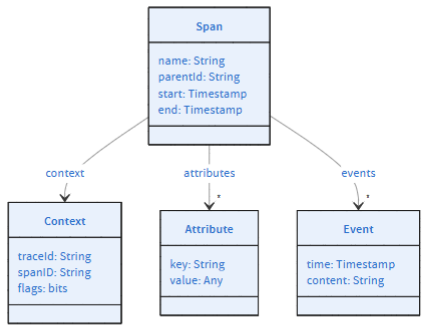
\includegraphics[width=0.3\linewidth]{content/chapters/images/2026-05-10-09-11-00.png}
  \end{minipage}
\end{center}


\section{Metrics}

A metric is a measurement of a service captured at runtime.
Metric event: measure values, timestamps and other metadata (i.e. Attributes).

Capture a measurement: Name, Kind, Unit, Description.

\subsection{Metric kind}

\begin{itemize}
  \item Counter: A value that accumulates over time
  \item UpDownCounter: A value that accumulates over time, but can also go down again, e.g. queue length
  \item Gauge: Measures a current value at the time it is read
  \item Histogram: A client-side aggregation of values, such as request latencies
\end{itemize}

Asynchronous: used if you access availablt only to the aggregated/current value

\paragraph{Entities Example}

App, browser, container, host, process, thread, service, etc.

\paragraph{Metrics examples}

For entity process:

\begin{table}[h!]
  \renewcommand{\arraystretch}{1.4}
  \centering
  \begin{tabular}{l c c c}
    \toprule
    \textbf{Name}   & \textbf{Type} & \textbf{Unit} & \textbf{Description}                    \\
    \midrule
    cpu time        & Counter       & s             & Total CPU seconds (by mode)             \\
    cpu utilization & Gauge         & l             & $\frac{\Delta time}{(elapsed * \#CPU)}$ \\
    memory usage    & UpDownCounter & by            & Amount of physical memory in use        \\
    \bottomrule
  \end{tabular}
\end{table}


For entity http\.server:

\begin{table}[h!]
  \renewcommand{\arraystretch}{1.4}
  \centering
  \begin{tabular}{l c c c}
    \toprule
    \textbf{Name}     & \textbf{Type} & \textbf{Unit} & \textbf{Description}                                     \\
    \midrule
    request duration  & Histogram     & s             & Duration of requests (attributes: method, url, ...)      \\
    active\_requests  & UpDownCounter & request       & Number of active requests (attributes: method, url, ...) \\
    request body size & Histogram     & by            & Payload size in bytes (attributes: method, url, ...)     \\
    \bottomrule
  \end{tabular}
\end{table}

\begin{flushleft}
  \begin{minipage}[t]{0.57\linewidth}

    \paragraph{Metric Example}

    \begin{itemize}
      \item Resource: namespace: my-site, name: frontend-web, id:http-server-136
      \item Metric: active\_requests
      \item Data point: value: 35, method: GET, url: /index.html
    \end{itemize}
  \end{minipage}%
  \hfill
  \begin{minipage}[t]{0.4\linewidth}
    \paragraph{Model}
    \centering
    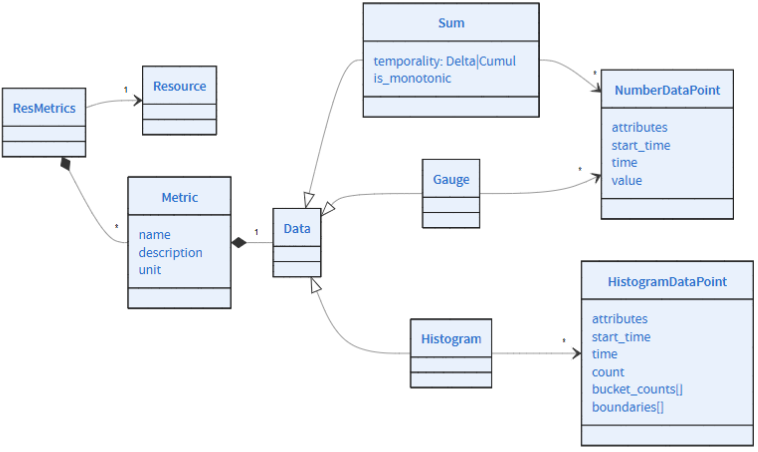
\includegraphics[width=0.7\linewidth]{content/chapters/images/2026-05-10-10-55-29.png}
  \end{minipage}
\end{flushleft}


\section{Profiling}
A running program consumes computational resources such as
memory, CPU cycles, and elapsed time.
To \textbf{profile} a program is to measure the consumption of such
resources by specific elements of the program.

\subsection{Why profiling?}
Profiling means:

\begin{itemize}
  \item make program more efficient
  \item developers more productive
  \item by identifying which program elements to optimize
\end{itemize}

The risk without profiling is to waste time in optimizing a
method consuming few resources resulting in little impact.

\subsection{Sampling vs. Tracing}
Two main approaches to collect profiling data: \textbf{Sampling}, an external harness samples the status of the program and
\textbf{Tracing}, an instrumented program emits samples during execution.

\subsubsection{Sampling}
Execution sampling providea an approximation of CPU
profiling.

\begin{itemize}
  \item Periodically interrupts the program (e.g., every 1ms)
  \item Records what the CPU is doing at that moment
  \item Low overhead, Works in production
  \item Not perfectly precise, but statistically accurate
\end{itemize}

\subsubsection{Tracing}

Tracing - a.k.a. instrumentation profiling - records function
calls (all or selected ones).

\begin{itemize}
  \item High detail (exact timings, call counts)
  \item Higher overhead
  \item Can distort performance
\end{itemize}

\subsection{Profile Types}
\begin{itemize}
  \item On-CPU
  \item Stall cycles: block on processor or hardware resources — typically memory I/O
  \item Memory: events related to memory growth e.g. malloc(), mmap(), etc.
  \item I/O: issuing of I/O, such as file system, storage device, and network
  \item Off-CPU: time spent while a thread is blocked, not running on a CPU (off-CPU time), e.g., waiting on I/O, locks, timers, a turn on-CPU, waiting for paging or swapping.
\end{itemize}

\subsection{Flamegraph}

\begin{center}
  \begin{minipage}{0.65\linewidth}
    Collection of stack samples represented as a column of boxes, each box represents a function (a stack frame).


    The y-axis shows the stack depth, from root at the bottom to leaf at the top. The top box is the function that was on-CPU


    The x-axis spans the stack trace collection (not time passing). Ordering is alphabetical on the function names.
    When identical boxes are adjacent, they are merged.


    The width of box is the frequency at which that function was present in samples.
    Functions with wide boxes were more present in the stack traces than those with
    narrow boxes, in proportion to their widths.

    The background color is random to help the eye differentiate boxes.
  \end{minipage}%
  \hfill
  \begin{minipage}{0.3\linewidth}
    \centering
    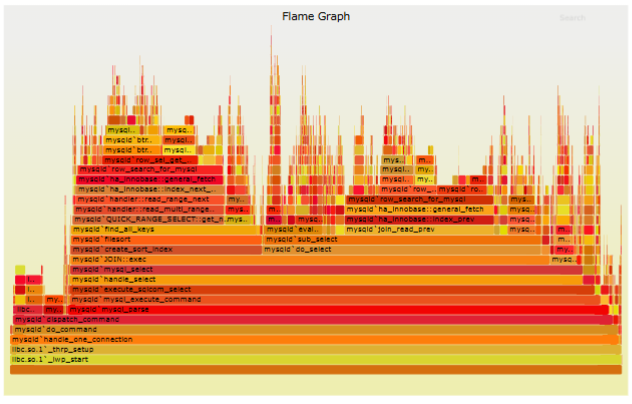
\includegraphics[width=\linewidth]{content/chapters/images/2026-05-10-11-11-15.png}
    captionof{figure}{Example of flamegraph}
  \end{minipage}
\end{center}


\subsubsection{Flamegraph interpretation}

The top is the function that was on-CPU when the stack trace was collected.
Look for large plateaus along the top edge: this means a single function was frequently
running on-CPU. Reading top down shows ancestry. Reading bottom up shows code flow and the bigger picture

The width of function boxes can be directly compared, if a function box is wider than another, this may be because it consumes more CPU
per function call or that the function was simply called more often.

Major forks in the flame graph can indicate, a logical grouping of code (work in stages), a conditional statement.

\section{Java Flight Recorder (JFR)}
JFR is a low-overhead profiling and monitoring system built
into the JVM. It records events about CPU, memory, GC, threads, I/O, and
JVM internals. Data is stored in a compact .jfr file for later analysis.
It supports both: continuous production monitoring and short profiling sessions.

\subsection{Collected Events}

\begin{itemize}
  \item JVM Internals (e.g. CPU, Threads, Monitors)
  \item Profiling (execution sampling)
  \item Garbage Collection
  \item Memory (object allocation)
  \item Exception
  \item I/O
  \item Class loading
\end{itemize}

\subsection{JFT settings}
Two predefined settings:

\begin{itemize}
  \item default: No jdk.ExecutionSample; Focus on: GC, locks, I/O, JVM internals; Very low overhead
  \item profile: Enables: jdk.ExecutionSample + allocation profiling; Higher overhead (~1-2\%); Suitable for flamegraphs
\end{itemize}

\paragraph{JFR profiling session example}

An app is run with JFR started from begin:

\begin{center}
  \begin{minipage}{0.3\linewidth}
    \centering
    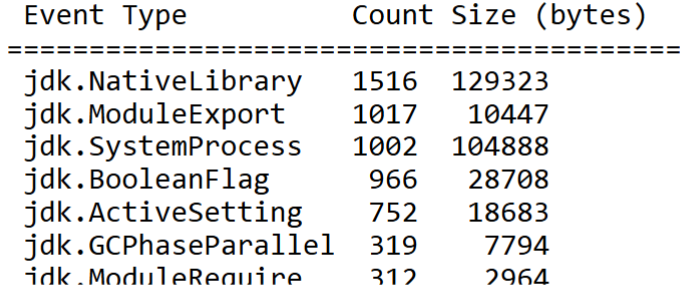
\includegraphics[width=\linewidth]{content/chapters/images/2026-05-10-11-22-36.png}
  \end{minipage}%
  \hfill
  \begin{minipage}{0.65\linewidth}
    \begin{minted}[breaklines]{java}
java \
    -XX:StartFlightRecording=filename=profiling-recording.jfr
    -cp target/classes \
    it.polito.swda.profiling.Example

jfr summary profiling-recording.jfr
\end{minted}
  \end{minipage}
\end{center}







